\documentclass[10pt]{beamer}
%%% Pour le français %%%
\usepackage[utf8]{inputenc}
\usepackage[T1]{fontenc}
\usepackage[french]{babel}
%%%%%%%%%%%%%%%%%%%%%%%%
% \usepackage{fancyhdr} % En-tête et pied de page personnalisés
\usepackage{listings} % Pour du beau code coloré
\usepackage{minted}
%%%% Pour des maths %%%%
\usepackage{mathtools} % Pour pleins de commandes avec des maths
\usepackage{amssymb} % Pour les symboles
\usepackage{amstext} % Pour utiliser \text
% \usepackage{mathrsfs} % 3 fonts pour les 26 lettres
% \usepackage{amsthm} % Custom des theoremes
% \usepackage{tikz} % Pour des graphiques
\usepackage{stmaryrd} % Pour les double crochets, parenthèses etc..
\usepackage{gensymb} % Pour des symboles tels que °, perthousand, ...
%%%%%%%%%%%%%%%%%%%%%%%%
% \usepackage{layout} % Pour afficher le gabarit de mise en page
% \usepackage{geometry} % Pour régler les marges
% \usepackage{setspace} % Pour modifier l'interligne
% \usepackage{ulem} % Pour souligner et barrer du texte
%%% Pour des polices %%%
% \usepackage{bookman}
% \usepackage{charter}
% \usepackage{newcent}
% \usepackage{lmodern}
% \usepackage{mathpazo}
% \usepackage{mathptmx}
%%%%%%%%%%%%%%%%%%%%%%%%
% \usepackage{url} % Pour citer des urls
\usepackage{graphicx} % Pour travailler sur des image
% \usepackage{color} % Pour manipuler les couleurs et colorer le texte
\usepackage{enumitem}
\usepackage{tabulary}

\title[TIPE — Problème de tournée des véhicules]{TIPE \\ Problème de tournée des véhicules}

\author{WILLEM Logan \\ \  \\Numéro de candidat: 1210 \\ \  \\ \insertframenumber / \inserttotalframenumber}
\date{2020 / 2021}

\lstset{basicstyle=\ttfamily}

\mode<presentation>

\usepackage{lastpage}

\useoutertheme[footline=authortitle,subsection=false]{miniframes}
\useinnertheme{circles}
\usecolortheme{whale}
\usecolortheme{orchid}

\definecolor{beamer@blendedblue}{rgb}{0.137,0.466,0.741}
\definecolor{titleColor}{RGB}{102,153,255}
\definecolor{textColor}{RGB}{60,60,60}
\definecolor{frametitlec}{RGB}{17,59,94}

\setbeamercolor{titlelike}{bg=titleColor}
\setbeamercolor{titlelike}{parent=structure}
\setbeamercolor{title}{fg=black}
\setbeamercolor{item}{fg=black}
\setbeamercolor{normal text}{fg=textColor}
\setbeamertemplate{background canvas}[vertical shading][top=cyan!7!white,bottom=cyan!2!white]
\setbeamertemplate{blocks}[rounded][shadow=true]
\setbeamercolor{prop_low}{bg=red!10,fg=black!90}
\setbeamercolor{prop_up}{fg=white,bg=red!90}
\setbeamercolor{data_low}{bg=gray!10,fg=black!90}
\setbeamercolor{data_up}{fg=white,bg=gray!90}

\setbeamercolor{frametitle}{fg=white,bg=frametitlec!95}

\setbeamerfont{frametitle}{size=\small}

\setbeamertemplate{navigation symbols}{}

% Pour élargir la surface utile dans beamer
\newenvironment{changemargin}[2]{
\begin{list}{}{
    \setlength{\topsep}{0pt}
    \setlength{\leftmargin}{#1}
	\setlength{\rightmargin}{#2}
 	\setlength{\listparindent}{\parindent}
    \setlength{\itemindent}{\parindent}
    \setlength{\parsep}{\parskip}
	}\item[]}{\end{list}}

\setcounter{tocdepth}{2}

\begin{document}
	\begin{frame}[plain]
		\maketitle
	\end{frame}

	\begin{frame}[plain]
		\tableofcontents
	\end{frame}

	\section{Optimisation et problème VRP}
	   
	\subsection{L'optimisation combinatoire}
	\subsubsection{Qu'est ce que l'optimisation combinatoire?}
	\begin{frame}
		\frametitle{L'optimisation combinatoire — Qu'est-ce que c'est?}
		\begin{center}
			Qu'est-ce que l'optimisation combinatoire? \\ \  \\
			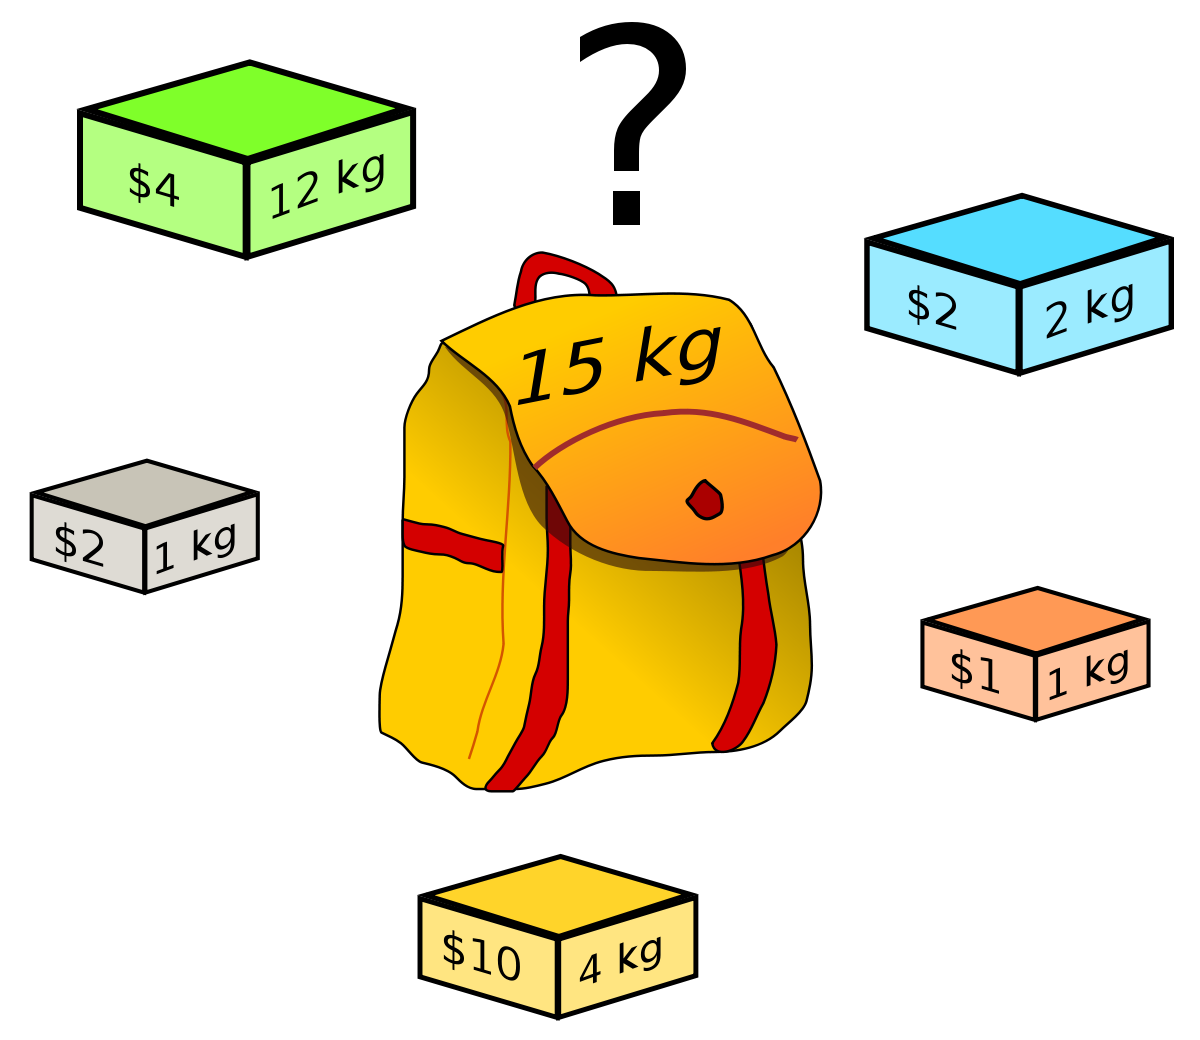
\includegraphics[scale=0.15]{image/probleme_du_sac_a_dos.png}
		\end{center}
	\end{frame}
	
	\subsubsection{Quelques exemples}

	\begin{frame}
		\frametitle{L'optimisation combinatoire — Quelques exemples}
		\underline{Quelques problèmes d'optimisation combinatoire}:
		\pause%
		\begin{itemize}[label=—]
			\item \textbf{Le voyageur de commerce}
		\end{itemize}
		\  \\
		\begin{center}
			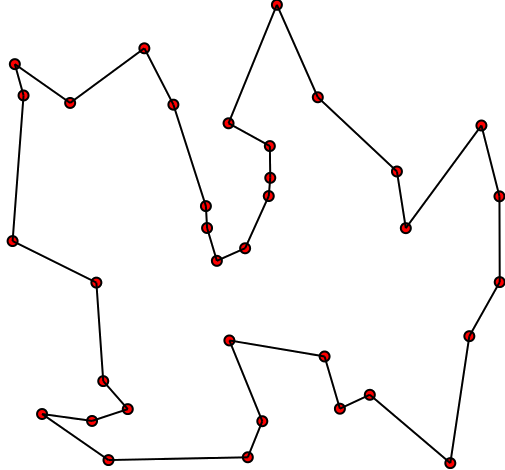
\includegraphics[height=4.5cm,width=4.5cm]{image/voyageur_de_commerce.png}
		\end{center}
	\end{frame}

	\begin{frame}
		\frametitle{L'optimisation combinatoire — Quelques exemples}
		\underline{Quelques problèmes d'optimisation combinatoire}:
		\begin{itemize}[label=—]
			\item Le voyageur de commerce
			\item \textbf{\textit{Bin packing}}
		\end{itemize}
		\begin{center}
			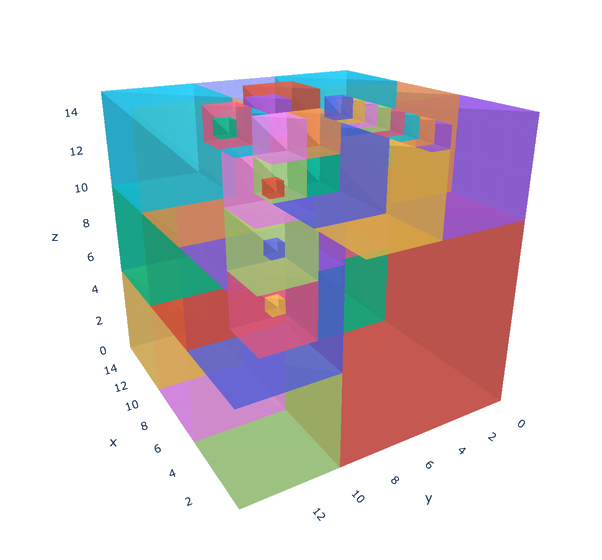
\includegraphics[scale=1]{image/bin_packing.png}
		\end{center}
	\end{frame}

	\begin{frame}
		\frametitle{L'optimisation combinatoire — Quelques exemples}
		\underline{Quelques problèmes d'optimisation combinatoire}:
		\begin{itemize}[label=—]
			\item Le voyageur de commerce
			\item \textit{Bin packing}
			\item \textbf{Tournée des véhicules}
		\end{itemize}
		\begin{center}
			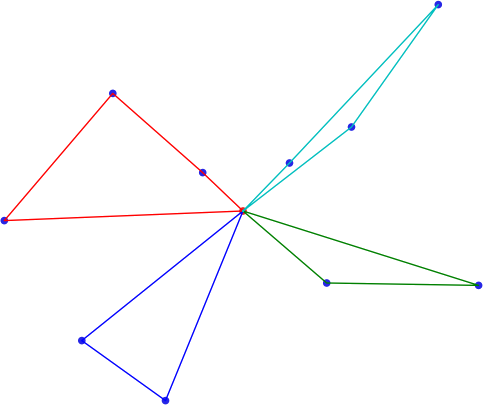
\includegraphics[scale=1.75]{image/tournee_des_vehicules.png}
		\end{center}
	\end{frame}

	\subsection{Problème de tournée des véhicules}

	\subsubsection{Contexte}
	
	\begin{frame}
		\frametitle{Problème de tournée des véhicules — Contexte}
		Le problème de tournée des véhicules (VRP:\textit{Vehicule Routing Problem}) consiste en la minimisation du coût total (en distance par exemple) de la tournée de tous les véhicules, ayant pour objectif de livrer un nombre défini de clients.
		\begin{center}
			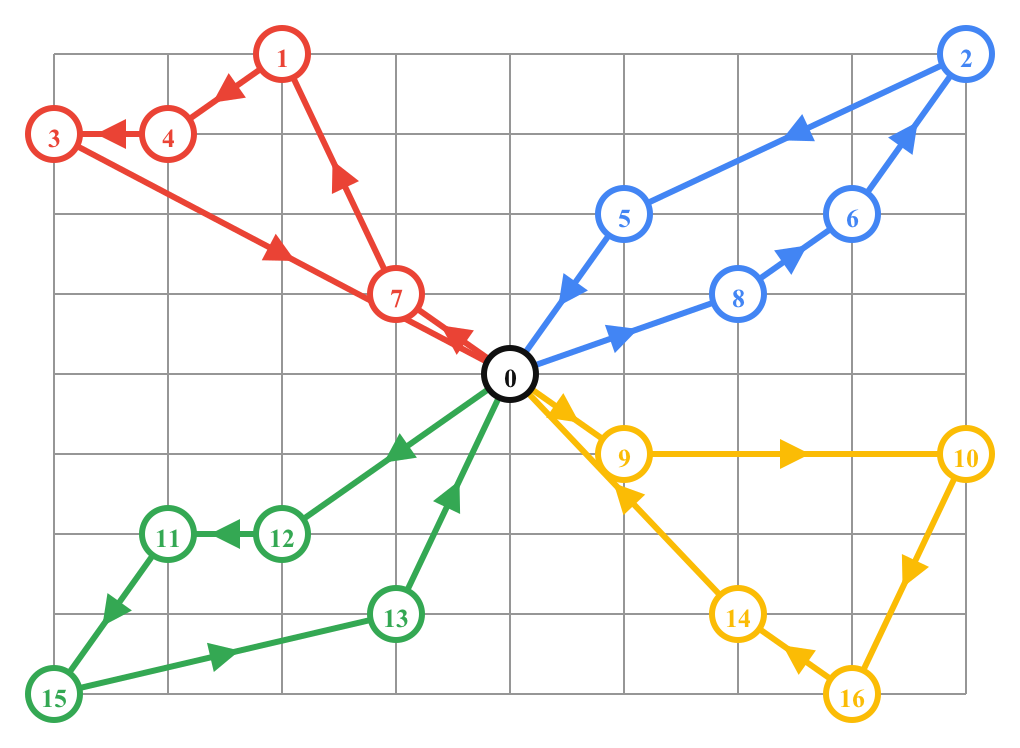
\includegraphics[scale=0.25]{image/vrp.png}
		\end{center}
	\end{frame}

	\subsubsection{Ancrage à la vie réelle}

	\begin{frame}
		\frametitle{Problème de tournée des véhicules — Ancrage à la vie réelle}
		\begin{figure}
			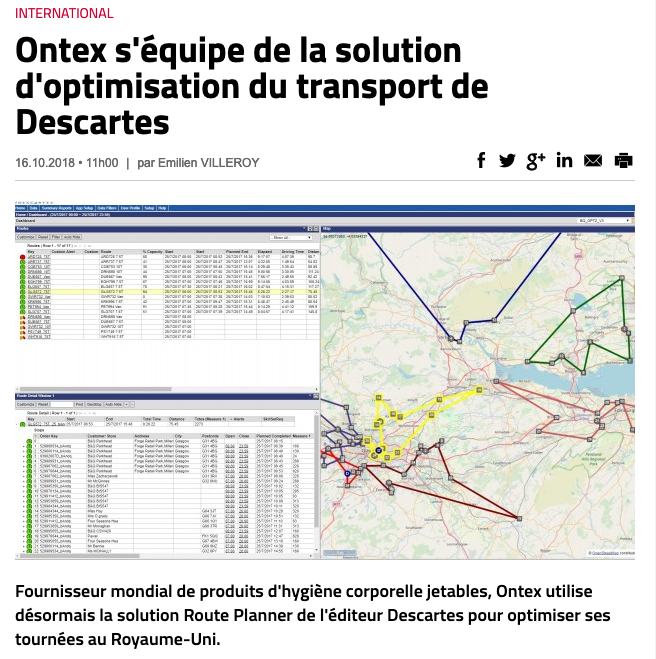
\includegraphics[scale=1.25]{image/Exemple_concret.png}
		\end{figure}		
	\end{frame}
	
	\subsubsection{Variantes}
	
	\begin{frame}
		\frametitle{Problème de tournée des véhicules — Variantes}
		\underline{Différentes variantes du problème de tournée des véhicules}
		\begin{itemize}[label=—]
			\item Classique (VRP)\pause%
			\item Contrainte de capacité (CVRP)\pause%
			\item Dép\(\hat{o} \)ts multiples (MDVRP)\pause%
			\item Retours des colis (VRPPD et VRPB)\pause%
			\item \dots 
		\end{itemize}
		\ \newline Je me suis intéressé à la version classique afin de m'approprier au mieux le problème.
	\end{frame}
	
	\subsubsection{Pourquoi utiliser une résolution approchée?}

	\begin{frame}
		\frametitle{Problème de tournée des véhicules — Pourquoi utiliser une résolution approchée?}
		Deux choix pour le \underline{premier} camion pour chaque client: ``OUI'' ou ``NON''
		\pause%
		\begin{center}
			\(2^n\) possibilités
		\end{center}
		\pause%
		Le sens importe peu:
		\begin{center}
			\(2^{n-1}\) possibilités
		\end{center}
		\pause%
		\  \\ Pour \underline{tous} les trajets, il existe \underline{au moins} \(2^{n-1}\) possibilités: \pause%
		\begin{center}
			complexité \textbf{exponentielle}
		\end{center}
	\end{frame}

	\section{Première résolution}

	\subsection{L'algorithme de Clarke et Wright}

	\begin{frame}
		\frametitle{L'algorithme de Clarke et Wright}
		\begin{beamerboxesrounded}[upper=data_up,lower=data_low,shadow=true]{Données}
			\begin{itemize}[label=-]
				\item Un point \(D\) de coordonnées \((0,0)\): le dép\(\hat{o} \)t
				\pause%
				\item Une famille de points \((i_1,\ldots ,i_n) \in {(\lbrack-100,100\rbrack^2)}^n\) pour un certain \(n \in \lbrack2,+\infty\lbrack \) représentant les clients
				\pause%
				\item Une fonction \(d\) qui calcule la distance entre deux points.
				\pause%
			\end{itemize}
		\end{beamerboxesrounded}\ \newline
		\underline{Remarque}: Dans cette méthode de résolution, le nombre de véhicules n'est pas fixé. C'est l'algorithme qui décide du nombre optimal de véhicules à utiliser. 
	\end{frame}

	\begin{frame}
		\frametitle{L'algorithme de Clarke et Wright}
		\begin{definition}[Fonction \textit{gain}]
			Fonction \(s \): calcule le gain après raccord de deux routes. \\Pour deux points \(i\) et \(j\), \(s\) calcule la différence de distance entre le chemin \\ \(D- i - D \) + \(D-j-D \) qui vaut \(2d(D,i) + 2d(j,D)\) au chemin\\ \(D-i-j-D \) de distance \(d(D,i) + d(i,j) + d(j,D)\)
		\begin{align*}
			s(i,j) &= 2d(D,i) + 2d(j,D) - \lbrack d(D,i) + d(i,j) + d(j,D)\rbrack \\
			s(i,j) &= d(D,i) + d(j,D) - d(i,j)
		\end{align*}
		\end{definition}
		\pause%
		\begin{tabular}{cccc}
			\; \; \; \;
			&
			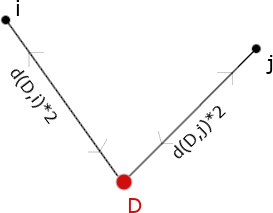
\includegraphics[scale=1.5]{image/did+djd.png}
			&
			\; \; \; \;
			\pause%
			&
			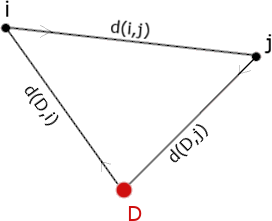
\includegraphics[scale=1.5]{image/dijd.png}			
		\end{tabular}
	\end{frame}

   \begin{frame}
	\frametitle{L'algorithme de Clarke et Wright}
		\underline{L'algorithme comporte deux étapes majeures}:
		\begin{itemize}[label=—]
			\item \textbf{Étape 1: Calcul des bénéfices}
			\  \\ Calcul la liste des bénéfices \(s_{ij}\) pour \(i,j \in \llbracket 1,n \rrbracket \) distincts
		\end{itemize}
	\end{frame}

	\begin{frame}
		\frametitle{L'algorithme de Clarke et Wright}
		\underline{L'algorithme comporte deux étapes majeures}:
		\begin{itemize}[label=—]
			\item Étape 1: Calcul des bénéfices
			\  \\ Calcul la liste des bénéfices \(s_{ij}\) pour \(i,j \in \llbracket 1,n \rrbracket \) distincts
			\item \textbf{Étape 2: Fusion des routes}
			\  \\ Fusion des routes si celles-ci peuvent l'être, dans l'ordre donné par la liste précédente
		\end{itemize}
	\end{frame}

	\subsection{Résultats}

	\begin{frame}
		\frametitle{Résultats}
		\begin{center}
			\begin{tabular}{c}
				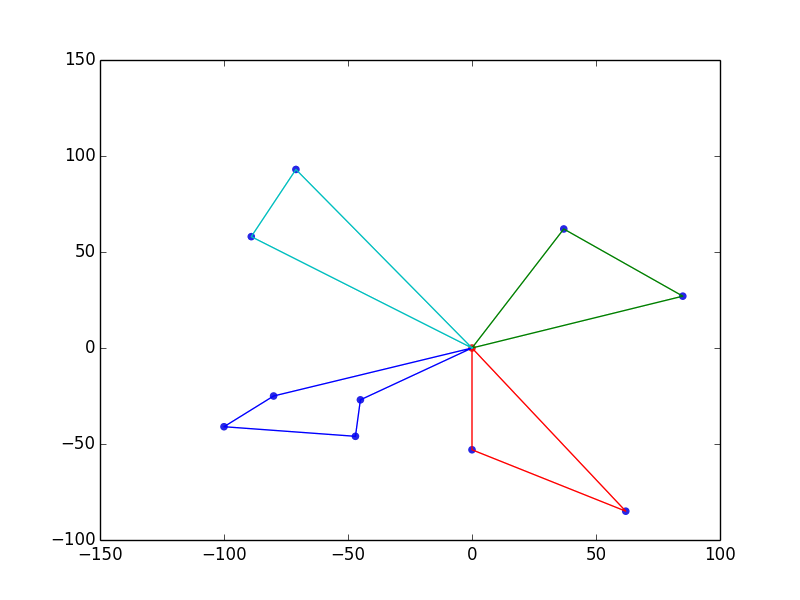
\includegraphics[scale=0.35]{image/CasParfait.png}
				\\
				Solution satisfaisante d'un problème
			\end{tabular}
		\end{center}
	\end{frame}

	\subsection{Insuffisance de l'algorithme}
	   
	\begin{frame}
		\frametitle{Insuffisance de l'algorithme}
		\begin{center}
			Exemples de résultats insatisfaisants
			\begin{tabular}{c c}
				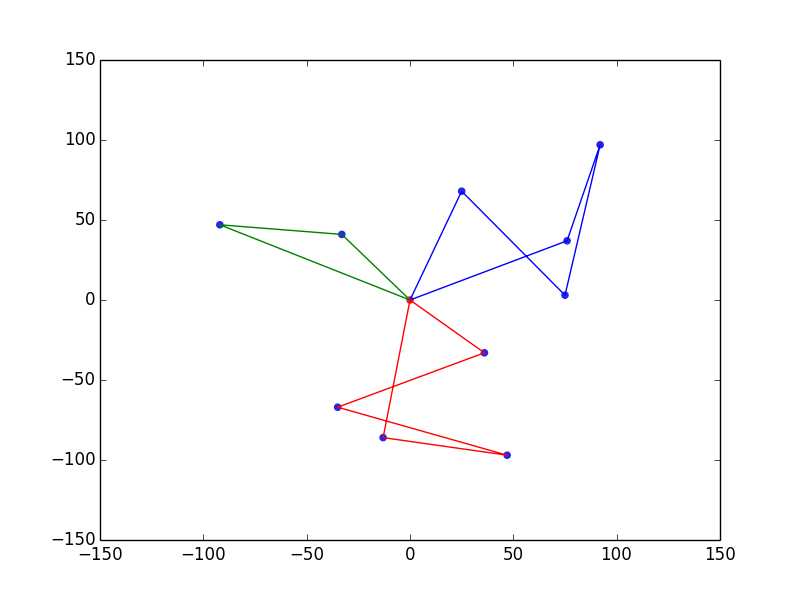
\includegraphics[scale=0.25]{image/Cas_avant_2-opt.png} & 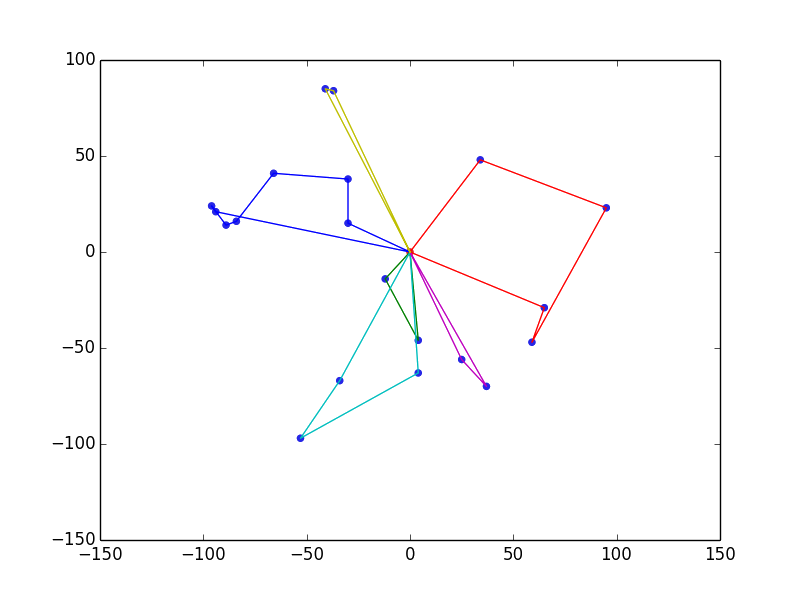
\includegraphics[scale=0.25]{image/Cas_avant_2opt_n2_1224.png}
				\\
				Pour \(n = 10 \) & Pour \(n = 20 \)
			\end{tabular}
		\end{center}
	\end{frame}

	\section{Le 2-opt}

	\subsection{Principe du 2-opt}

	\begin{frame}
		\frametitle{Principe du 2-opt}
			\begin{center}
				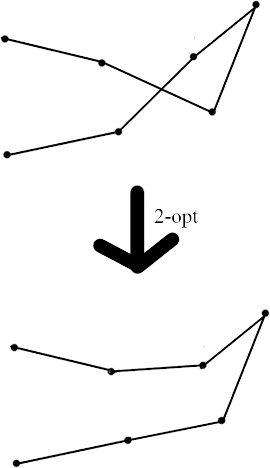
\includegraphics[scale=1]{image/principe-2-opt.png}
				\  \\Principe du 2-opt\\Suppression des liaisons sécantes
			\end{center}
	\end{frame}
	\begin{frame}
		\frametitle{Principe du 2-opt}
		\begin{exampleblock}{\textbf{Exemple}}
			Soit un chemin \((a,c,b,d)\). Dans le graphe ci-dessous, on a:
			\[d(a,c) + d(b,d)\, >\, d(a,b) + d(c,d)\] Un changement va donc s'opérer: \((a,\textbf{c},\textbf{b},d) \rightarrow (a,\textbf{b},\textbf{c},d)\) \\
			\begin{center}
				\begin{tabular}{cc}
					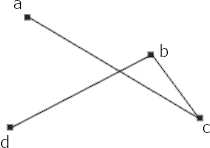
\includegraphics[scale=2]{image/acbd.png}
					& \pause%
					\quad \quad \quad 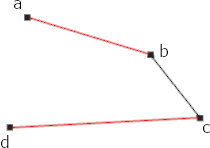
\includegraphics[scale=2]{image/abcd.png}
				\end{tabular}
			\end{center}
		\end{exampleblock}
	\end{frame}

	\subsection{Comparaison avec et sans 2-opt}
	
	\begin{frame}
		\frametitle{Comparaison avec et sans 2-opt}
		\begin{center}
		\textbf{10 clients}
		\end{center}
		\ \newline
		\begin{tabular}{cc}
			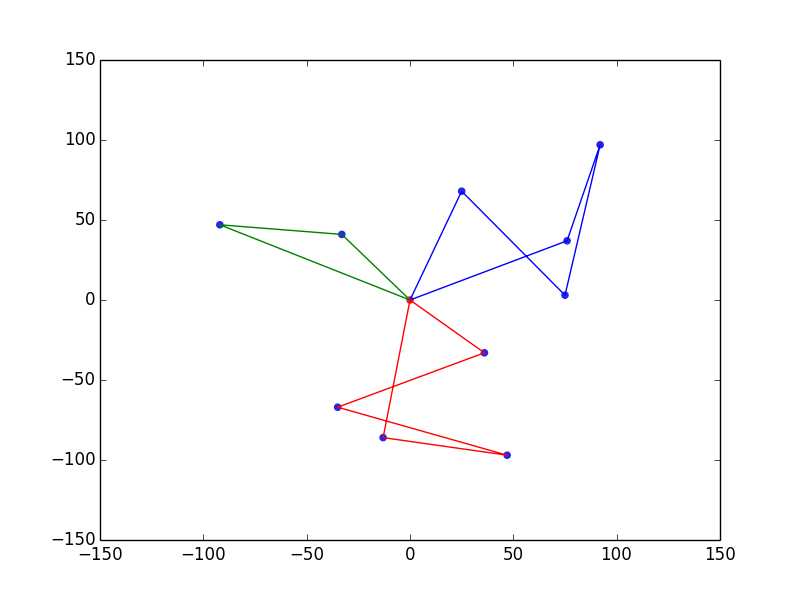
\includegraphics[scale=0.25]{image/Cas_avant_2-opt.png}
			&
			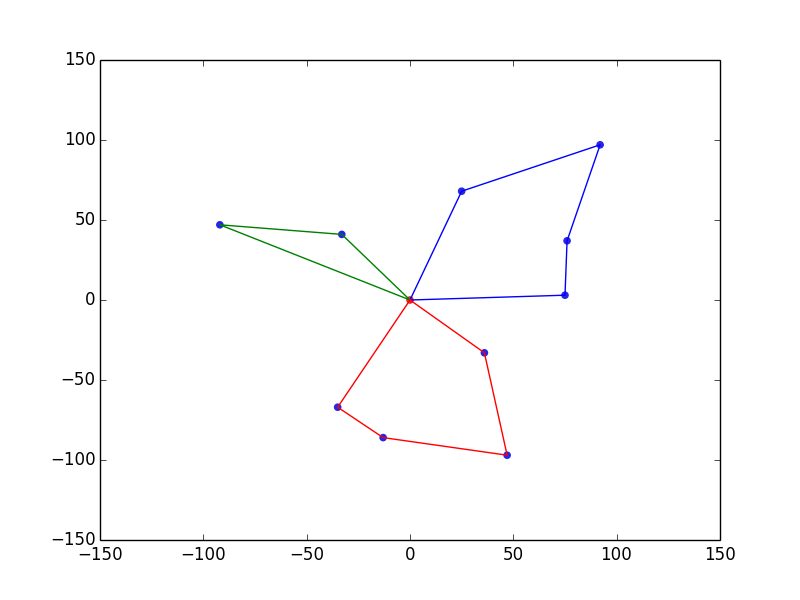
\includegraphics[scale=0.25]{image/Cas_apres_2-opt.png}
			\\                                                     
			Avant&Après
		\end{tabular}
	\end{frame}
	
	\begin{frame}
		\frametitle{Comparaison avec et sans 2-opt}
		\begin{center}
			\textbf{20 clients}
		\end{center}
		\ \newline
		\begin{tabular}{cc}
			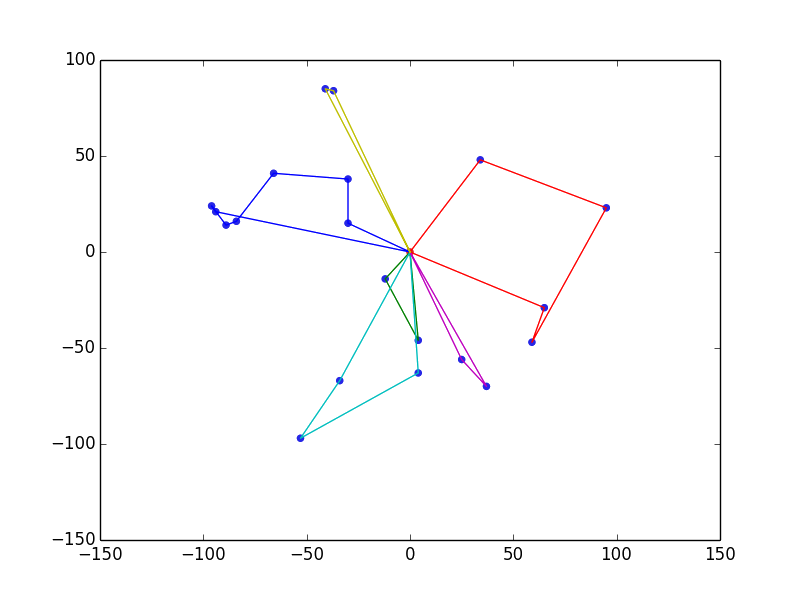
\includegraphics[scale=0.25]{image/Cas_avant_2opt_n2_1224.png}
			&
			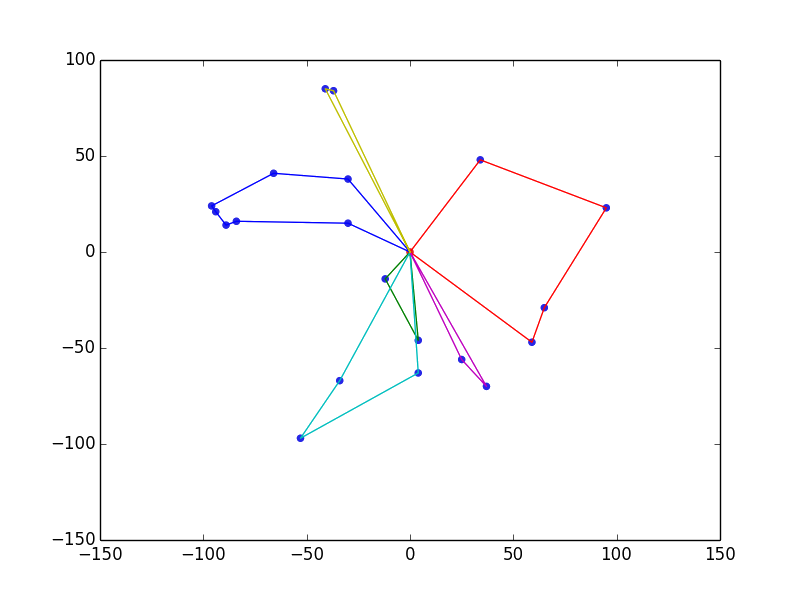
\includegraphics[scale=0.25]{image/Cas_apres_2opt_n2_1193.png}
			\\
			Distance: 1224km&Distance: 1193km
			\\                                                     
			Avant&Après
		\end{tabular}
	\end{frame}
	
	\section{L'opérateur inter-route}

	\subsection{Principe de l'opérateur}


	\begin{frame}
		\frametitle{Principe de l'opérateur}
		\underline{L'algorithme comporte trois étapes}:
		\begin{itemize}[label=—]
			\small{\item \textbf{Étape 1: Calcul des plus proches voisins pour chaque point}}
			\  \\ 
			\small{Calcul de la liste des plus proches voisins à chaque point pour chaque autre route déjà formée} \\ \  \\
		\end{itemize}
	\end{frame}

	\begin{frame}
		\frametitle{Principe de l'opérateur}
		\underline{L'algorithme comporte trois étapes}:
		\begin{itemize}[label=—]
			\small{\item Étape 1: Calcul des plus proches voisins pour chaque point
			\  \\ Calcul de la liste des plus proches voisins à chaque point pour chaque autre route déjà formée 
			\item \textbf{Étape 2: Calcul de l'optimisation engendré}
			\  \\ Calcul de la liste des gains (et/ou des pertes) par migration temporaire d'un point sur chaque autre route en fonction de la liste de l'étape 1.} \\ \  \\
		\end{itemize}	
	\end{frame}

	\begin{frame}
		\frametitle{Principe de l'opérateur}
		\underline{L'algorithme comporte trois étapes}:
		\begin{itemize}[label=—]
			\small{\item Étape 1: Calcul des plus proches voisins pour chaque point
			\  \\ Calcul de la liste des plus proches voisins à chaque point pour chaque autre route déjà formée 
			\item Étape 2: Calcul de l'optimisation engendré
			\  \\ Calcul de la liste des gains (et/ou des pertes) par migration temporaire d'un point sur chaque autre route en fonction de la liste de l'étape 1.
			\item \textbf{Étape 3: Migrations des points}
			\  \\ La migration du point donnant le plus grand gain est faite définitivement. Puis on recommence à l'étape 1 tant que cette liste contient des gains.} \\ \  \\
		\end{itemize}	
	\end{frame}

	\subsection{Exemple d'utilisation}

	\begin{frame}
		\frametitle{Exemple d'utilisation}
		\begin{exampleblock}{\textbf{Exemple}: Solution de départ}
			\begin{center}
				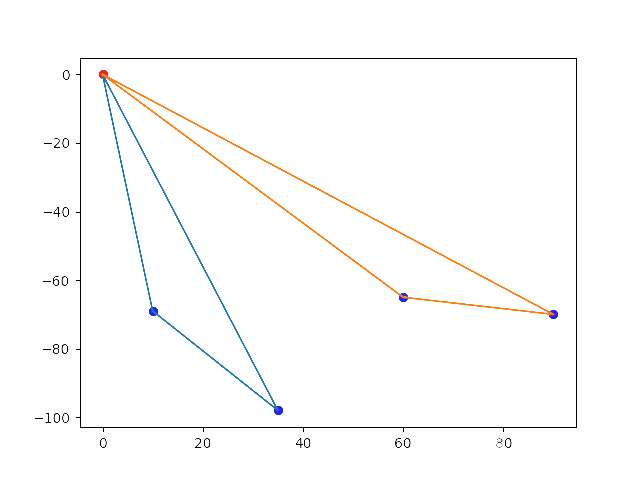
\includegraphics[scale = 0.46]{image/inter_route_1.png}  \\
				Distance: 445km
			\end{center}
		\end{exampleblock}
	\end{frame}

	\begin{frame}
		\frametitle{Exemple d'utilisation}
		\begin{exampleblock}{\textbf{Exemple}: Première exécution de l'opérateur}
			\begin{center}
				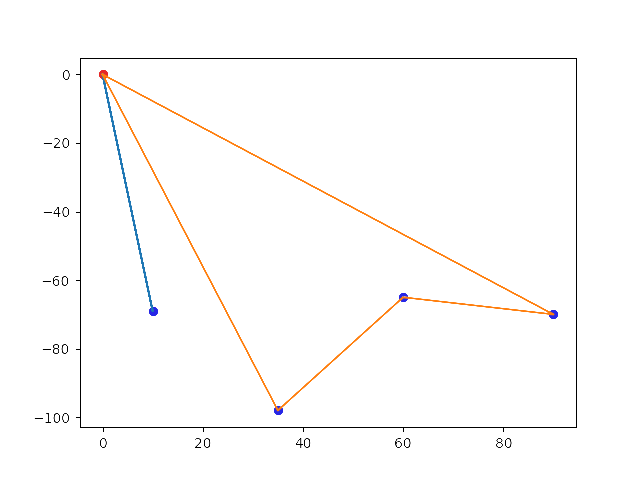
\includegraphics[scale = 0.46]{image/inter_route_2.png}  \\
				Distance: 429km
			\end{center}
		\end{exampleblock}
	\end{frame}

	\begin{frame}
		\frametitle{Exemple d'utilisation}
		\begin{exampleblock}{\textbf{Exemple}: Seconde exécution de l'opérateur}
			\begin{center}
				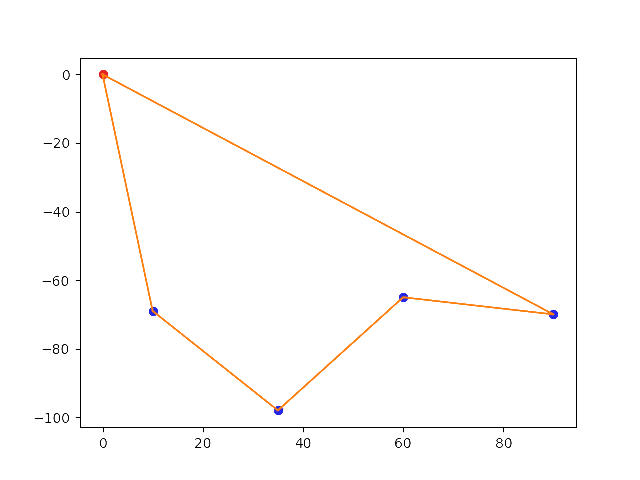
\includegraphics[scale = 0.46]{image/inter_route_3.png}  \\
				Distance: 382km
			\end{center}
		\end{exampleblock}
	\end{frame}

	\subsection{Comparaison avec et sans l'opérateur inter-route}

	\begin{frame}
		\frametitle{Comparaison avec et sans l'opérateur inter-route}
		\begin{center}
			\begin{tabular}{c c}
				\quad \quad \quad 2-opt & Opérateur inter-route + 2-opt  \\
				\quad \quad \quad 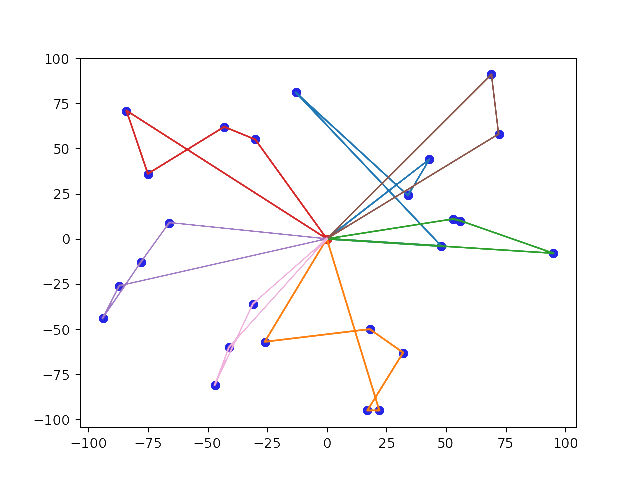
\includegraphics[scale=0.22]{image/2_sans_rien.png} \quad & 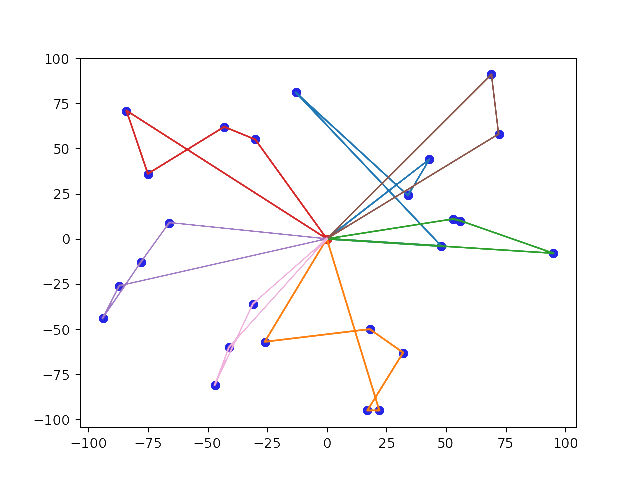
\includegraphics[scale=0.22]{image/2_sans_rien.png}  \\ 
				\quad \quad \quad \( \downarrow \) & \( \downarrow \)  \\
				\quad \quad \quad 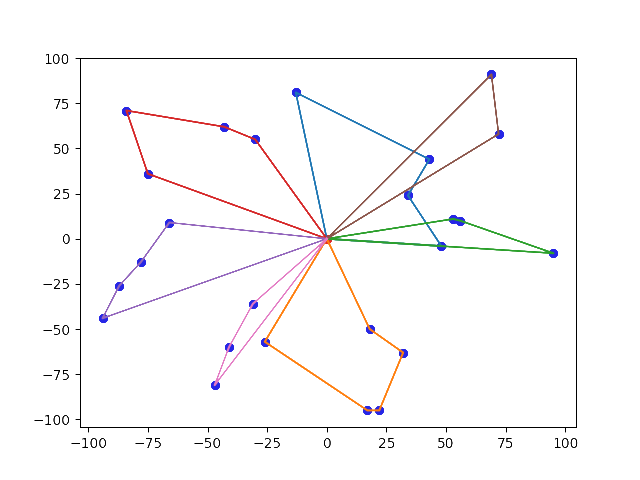
\includegraphics[scale=0.22]{image/2_deux_opt.png} \quad & 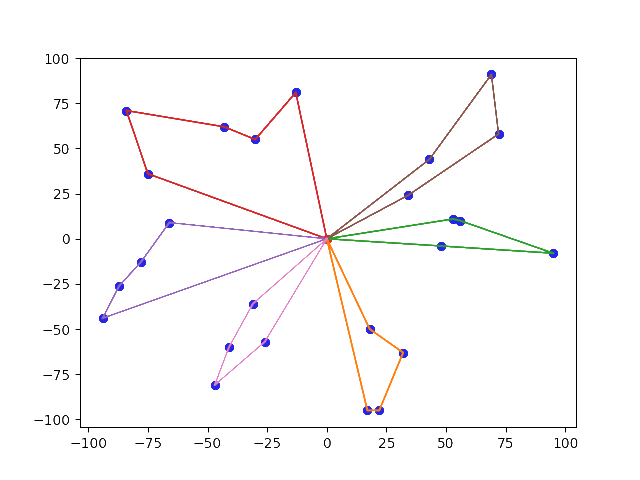
\includegraphics[scale=0.22]{image/2_bis_deux_opt.png}  \\
				\quad \quad \quad Distance: 1575km & Distance: 1429km
			\end{tabular}
		\end{center}
	\end{frame}

	\section{Résultats et limites}

	\subsection{Résultats}

	\begin{frame}
		\frametitle{Résultats}
		\begin{center}
			Moyenne des gains en fonction du nombre \( n \) de clients
			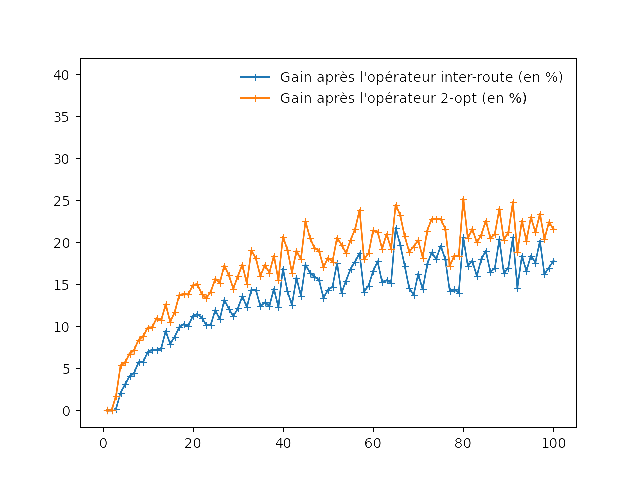
\includegraphics[scale=0.4]{image/gain_en_pourcent.png}
		\end{center}
		\small{Moyenne avec l'opérateur inter-route seulement (à partir de \( n=40 \)): 16.6 \%  \\
		Moyenne avec les opérateurs inter et intra route (à partir de \( n=40 \)): 20.6 \%  \\
		Meilleure optimisation après les deux opérateurs: 35 \% (pour \( n = 88 \))}
	\end{frame}

	\subsection{Complexité de l'algorithme}

	\begin{frame} 
		\frametitle{Complexité de l'algorithme}
		\begin{center}
			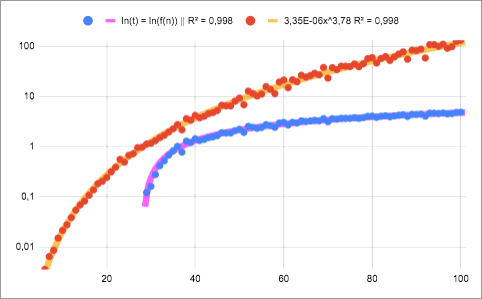
\includegraphics[scale=1.8]{image/complexite.png} \  \\ \  \\
			\( t = 3.35\times10^{ - 6}x^{3.78} \)
			\\ \  \\
			Complexité: \textbf{polynomiale}
		\end{center}
	\end{frame}

	\begin{frame}
		\frametitle{Complexité de l'algorithme}
		\begin{changemargin}{-1cm}{-0.5cm}
			\begin{tabular}{c c}
				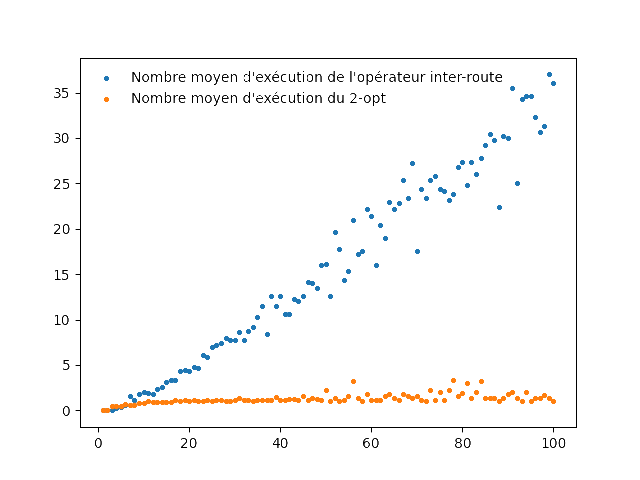
\includegraphics[scale=0.35]{image/nombre_exec.png} & 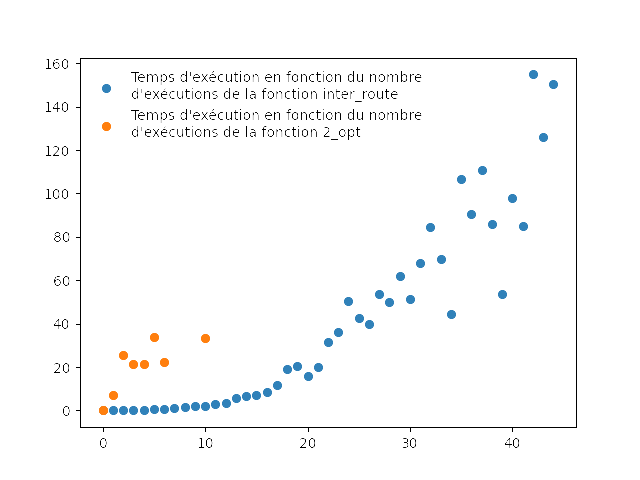
\includegraphics[scale=0.35]{image/temps_en_f_nb_inter_route.png} 
				\\
				\begin{tabular}{c}
					Nombre d'appels des opérateurs\\ en fonction de \( n \)	
				\end{tabular}
				& 
				\begin{tabular}{c}
					Temps d'exécution en fonction\\ du nombre d'exécutions des opérateurs 
				\end{tabular}
			\end{tabular}
		\end{changemargin}
	\end{frame}

	\subsection{Limites de l'algorithme}

	\begin{frame}
		\frametitle{Limites de l'algorithme}
		\begin{center}
			\textbf{Limite n\degree1: Ajout de contraintes} \  \\  \  \\
		Algorithme de Clarke et Wright introduit pour le problème VRP\@. \\ \  \\
		Donc \underline{non adapté} aux ajouts de contraintes.
		\end{center}
	\end{frame}
	
	\begin{frame}
		\frametitle{Limites de l'algorithme}
		\begin{center}
			\textbf{Limite n\degree1: Ajout de contraintes}
		\end{center}
		D'autres algorithmes permettent d'obtenir des solutions satisfaisantes:
		\begin{itemize}[label=\( \bullet \)]
			\pause%
			\item Recherche exacte:
				\begin{itemize}[label=–]
					\item Séparation et Évaluation (\textit{Branch and Bound})
				\end{itemize}
			\pause%
			\item Heuristiques:
				\begin{itemize}[label=–]
					\item \textit{Petal algorithm}
					\item \textit{Sweep algorithm}
				\end{itemize}
			\pause%
			\item Métaheuristiques:
				\begin{itemize}[label=–]
					\item Recherche Tabou (\textit{Tabu Search})
					\item Algorithme génétique (\textit{Genetic algorithm})
					\item Colonie de fourmis (\textit{Ant algorithm})
					\item GRASP (\textit{Greedy Randomized Adaptive Search Procedure})
				\end{itemize}
		\end{itemize}
	\end{frame}

	\begin{frame}
		\frametitle{Limites de l'algorithme}
		\begin{center}
			\textbf{Limite n\degree2: Algorithme glouton}
		\end{center}
		L'algorithme de Clarke et Wright est glouton: pour chaque étape, seul le plus grand bénéfice est considéré \\
		Aucune dégradation d'une solution n'est donc envisageable. \\
		\begin{center}
			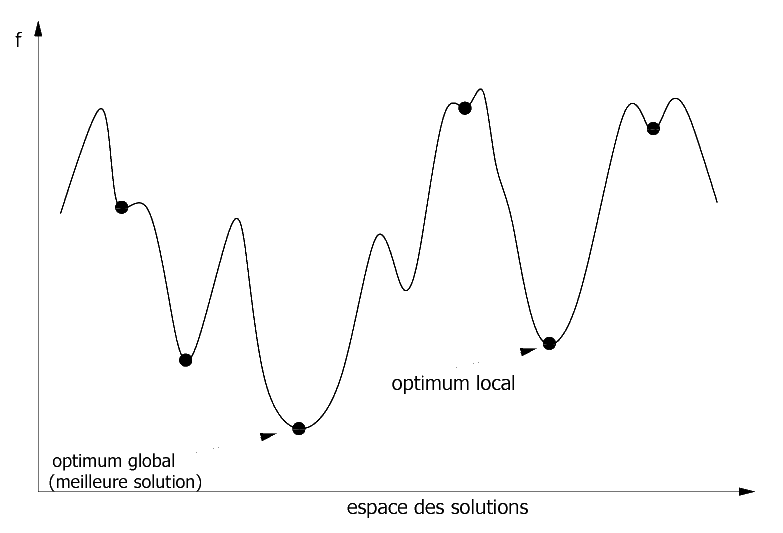
\includegraphics[scale=]{image/graph.png}
		\end{center}

	\end{frame}
	
	\begin{frame}
		\frametitle{Limites de l'algorithme}
		\begin{center}
			\textbf{Limite n\degree3: Long temps d'exécution}
		\end{center}
		\underline{Objectif}: Trouver des solutions en évitant la complexité exponentielle de l'algorithme naïf. \\ \  \\
		Sur le graphe représentant le \( t \) en fonction de \( n \): \( n = 100, \)\quad \( t \thickapprox 135\text{s} \) \  \\ \  \\
		Il serait donc difficile de résoudre des instances trop grandes (jusqu'à \( n = 30000 \)) \\ \  \\
		L'algorithme convient cependant a une utilisation ``normale'' (livraisons dans une zone géographique restreinte)
	\end{frame}

	\begin{frame}
		\frametitle{Limites de l'algorithme}
		\begin{center}
			\textbf{Limite n\degree4: Résultats non optimaux} 
			\  \\ 
			\  \\
			Instance A-n32-k5 
			\begin{tabular}{c c}
				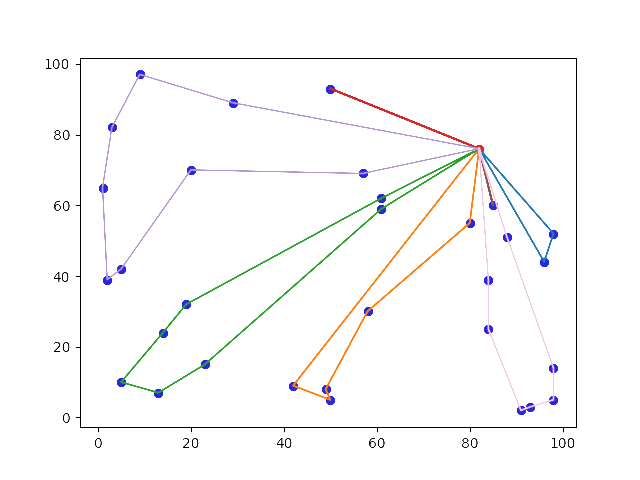
\includegraphics[scale=0.3]{image/A_n32_k5.png} & 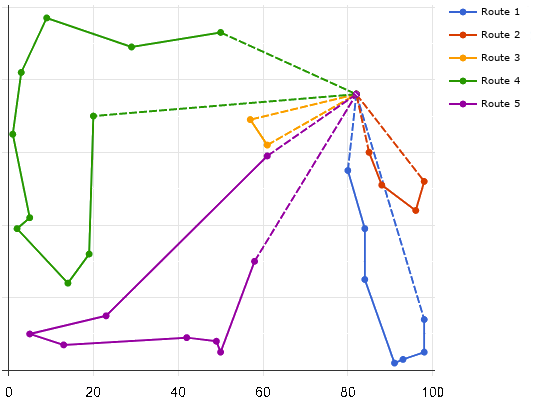
\includegraphics[scale=0.9]{image/A_n32_k5_optim.png} \\
				Distance: 945km & Distance: 784km
			\end{tabular}
		\end{center}	
	\end{frame}
	
	\begin{frame}
		\frametitle{Limites de l'algorithme}	
		\begin{center}
			\textbf{Limite n\degree4: Résultats non optimaux} 
			\  \\
			\  \\
			Instance A-n33-k5
			\begin{tabular}{c c}
				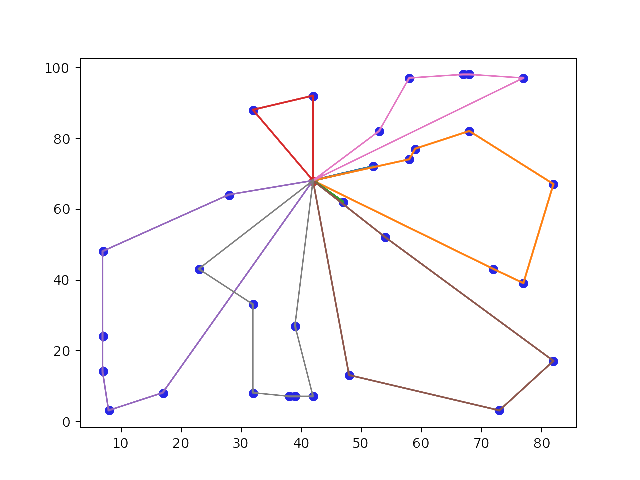
\includegraphics[scale=0.3]{image/A_n33_k5.png} & 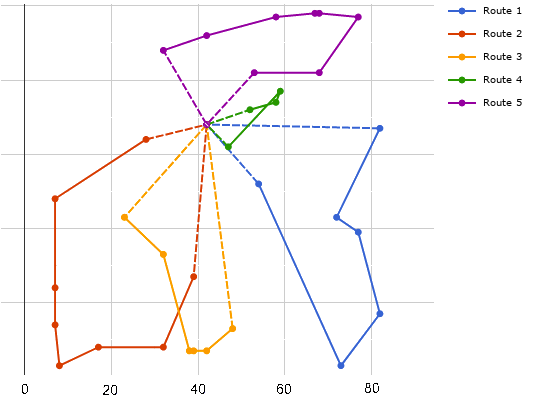
\includegraphics[scale=0.9]{image/A_n33_k5_optim.png} \\
				Distance: 784km & Distance: 661km
			\end{tabular}
		\end{center}
	\end{frame}

	\section*{\ }
	\subsection*{\ }

	\begin{frame}[plain]
		\begin{center}
			\Huge{\textbf{Conclusion}}
		\end{center}
		\  \\ Nous avons vu:
		\begin{itemize}[label=—]
			\item Les enjeux du problème \pause%
			\item Une première heuristique: celle de Clarke et Wright \pause%
			\item Une heuristique de recherche locale: le 2-opt \pause%
			\item Une heuristique d'optimisation inter-route \pause%
			\item Les résultats \pause%
			\item Les limites \pause% 
		\end{itemize}
		\  \\
		Il s'agirait désormais d'étendre la résolution du problème en y ajoutant des contraintes telles qu'une contrainte de capacité, ou de retour des marchandises. 
	
	\end{frame}

	\subsection*{\ }

	\begin{frame}[plain]
		\begin{center}
			\Huge{\textbf{Remerciements}}
		\end{center}
		{\small
		\  \\ \  \\Merci aux membres du jury pour leur écoute.\\ \  \\
		Merci à M. Bertault et M. Bouverot pour leur aide durant ces deux années.\\ \  \\
		Merci à M. Legrand-Lixon, agrégé de maths, pour l'orientation qu'il a donné à mon TIPE.\\ \  \\
		Merci enfin à M. Massoteau, ingénieur développeur chez Fastercom (et à son PDG, Romain Bonnifet), pour leur soutien et les différentes explications et aides fournies par appel visio. 
		}
	\end{frame}

	\subsection*{\ }
	
	\begin{frame}[plain]
		\begin{center}
			\Huge{\textbf{Annexe}} \\ Code complet
		\end{center}
	\end{frame}

	\section*{\ }

	\subsection*{\ }

	\begin{frame}[plain]
		\small{\inputminted{python}{python.py}}
	\end{frame}
	
	\subsection*{\ }

	\begin{frame}[plain]
		\footnotesize{\inputminted{python}{python2.py}}
	\end{frame}

	\subsection*{\ }

	\begin{frame}[plain]
		\footnotesize{\inputminted{python}{python3.py}}
	\end{frame}

	\section*{\ }

	\subsection*{\ }

	\begin{frame}[plain]
		\small{\inputminted{python}{python4.py}}
	\end{frame}

	\subsection*{\ }

	\begin{frame}[plain]
		\small{\inputminted{python}{python5.py}}
	\end{frame}

	\subsection*{\ }

	\begin{frame}[plain]
		\footnotesize{\inputminted{python}{python6.py}}
	\end{frame}

	\section*{\ }

	\subsection*{\ }

	\begin{frame}[plain]
		\tiny{\inputminted{python}{python7.py}}
	\end{frame}

	\subsection*{\ }

	\begin{frame}[plain]
		\footnotesize{\inputminted{python}{python8.py}}
	\end{frame}

	\subsection*{\ }

	\begin{frame}[plain]
		\tiny{\inputminted{python}{python9.py}}
	\end{frame}

	\section*{\ }

	\subsection*{\ }

	\begin{frame}[plain]
		\small{\inputminted{python}{python10.py}}
	\end{frame}

	\subsection*{\ }

	\begin{frame}[plain]
		\footnotesize{\inputminted{python}{python11.py}}
	\end{frame}

\end{document}